\section{Introduction}

\section{Patterns}

\subsection{Find-Fix-Verify}
The Find-Fix-Verify pattern was introduced by the Soylent paper. The pattern divide the overall task into three stages. During the Find stage, the workers will identify patches of work done by the crowd or create new patches. For example, the workers has to select a sentence which seems to be incorrect and will need further investigations during the Fix phase. Some workers will revise the identified patches and try to provide some alternatives. The last step of the pattern will present the generated alternatives during the Fix stage to a few new workers in a randomize order. The answer with the most votes (plurality voting) will be used to replace the identified patch during the first phase. The creators of the new suggestions will be suspended so that they can't vote for their own input. To illustrate the meaning of the Find-Fix-Verify pattern, the implementation of Soylent will be discussed (Figure \ref{fixfindverify}). The approach begins by splitting a text into paragraphs. During the Find stage, the workers has to identify candidate areas for shortening in each paragraph. If a certain number of workers has selected the same area then this patch goes to the next stage. Every worker in the Fix stage has to present a shorter version of the identified patch if possible. He has also the possibility to say that the text can't be reduced. During the last step, the crowd has to select rewrites which has significant spelling, style or grammar problems or change the meaning of the sentence significantly. At the end they remove these patches by majority voting.
\begin{figure}
\centering
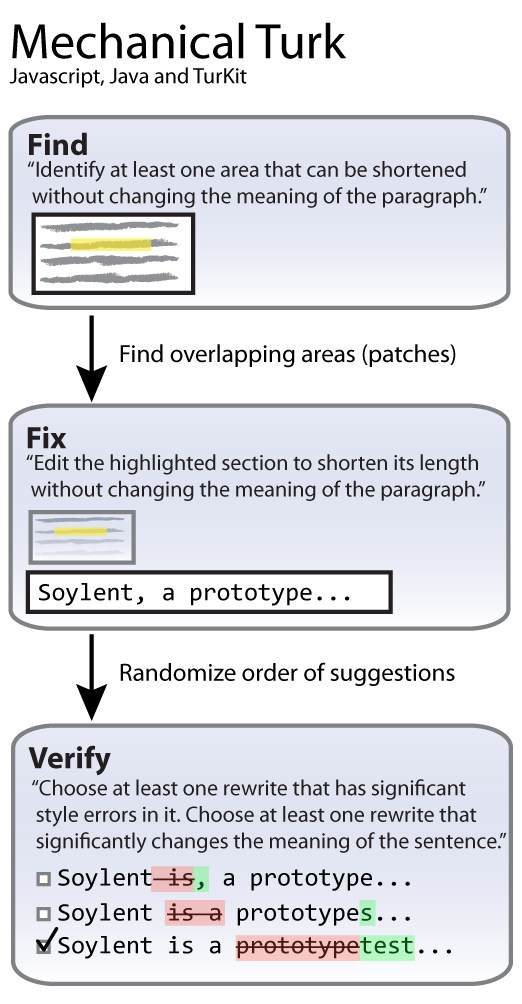
\includegraphics[scale=0.25]{images/soylent_system_overview.png}
\caption{Soylent Fix-Find-Verify pattern}
\label{fixfindverify}
\end{figure}

\subsection{Iterative}
Most of the published assignments on MTurk are independent, parallel tasks. But also iterative, sequential tasks can be useful. The authors of the TurKit paper implemented a tool which make iterative tasks possible. They developed an example application for creating an image description (Figure \ref{turkit}). During the first iteration, the worker will contribute the initial description of the provided image. The next iteration will show the initial description and a request to improve it. A few workers will evaluate the extension of the description by voting. If the extended description doesn't receive enough votes then the iteration will be ignored. The final description is generated after a fixed number of iterations. To make the iterative solution possible, the crash-an-rerun programming model was introduced by the authors of the paper. This model allows a script to be re-executed after a crash without generating costly side-effects. That means, if there is a crash during the second iteration of an iterative problem the first iteration will be skipped after re-running the script. TurKit is able to persist the state of the program and will never repeat the successfully completed task. This is helpful for prototyping algorithms.
\begin{figure}
\centering
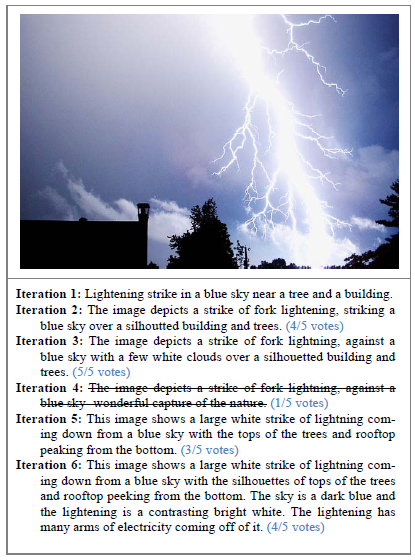
\includegraphics[scale=0.55]{images/turkit_description_example.png}
\caption{Iterative image description created by TurKit}
\label{turkit}
\end{figure}

\section{Design}
MTurk best practices, Iteration, Very important, Instructions are the key

\section{Hybrid}

\section{Quality control}

\subsection{Honey pots}

\section{Workflow}
The process of decomposing complex tasks into simpler ones is not always easy and need a lot of clarifications. The developers of the Turkomatic tool had an obvious idea and source the workflow decomposition out to the crowd. The workers should decide how the final workflow should look like and what are the single tasks. The system consists of two major parts. The meta-workflow
CrowdWeaver, CrowdForge

\section{Incentives}
ESP, Money, Financial Incentives and the ''Performance of Crowds''

